\chapter{Feasibility of Learning}\label{Sec:Feasibility of Learning}

No practical amount of data can distinguish between two distributions, thus instances of GBS can not be proven to come from GESIS. However, machine learning allows to infer the conditional probability of \textit{'GBS participant is representative'} given the survey data within a probabilistic framework. 

This leads to a binary classification task with GESIS as positive class and GBS as negative class, i.e. representative and non-representitve sample respectively. Discriminative learners will look for decision boundaries to distinguish the different views of GBS from GESIS in each of the four reference studies. False negatives are then more closely aligned with the target probability distribution. The process of classification is repeated until the learner starts fitting noise more than is warranted. To avoid overfitting, the learning objective needs to be refined as contingency tables lack proper interpretibility. An importance weighted adaption of cross-validation serves as model selection criterion. Given the imbalanced nature and size of GBS, learning is restrained to simpler algorithms with lesser degrees of freedom. The fraction of false positives in the result set of this procedure is kept as proxy measure for the subsequent method positive-unlabeled learning (PU learning). The development of classification models in this setting is often referred to as positive-unlabeled learning (Denis et al. 2005).


No practical amount of data can distinguish between two distributions, thus instances of GBS can not be proven to come from GESIS. However, machine learning allows to infer the conditional probability of \textit{'GBS participant is representative'} given the survey data within a probabilistic framework. A well-defined learning problem involves a number of design choices, including selecting the target function to be learned, a representation for this target function, and an algorithm to learn from the source of training experience [2]. This chapter covers the theoretical aspects of the MRS procedure introducing positive-unlabeled learning in addition to traditional machine learning.

\section{Terminology and Definitions}

Key terminology and destinctions made in the field of survey analytics are defined in this section. When learning from biased data, basic design issues and approaches to discriminative learning must be adjusted. The role of noise in the bias-variance decomposition will be analyzed and further broken down. Discriminative learning then uses techniques to address high variance.

\subsection{Sampling Bias}

Sampling bias is often referred to as selection bias or sample selection bias. I will stick to the more descriptive term sampling bias. It underlines the fact that the bias arises in how the data was sampled. Also, the use of the term becomes less ambiguous, because there exists another notion of selection bias in the context of model selection. This type of bias is usually referred to as bad generalization, where the performance of the selected hypothesis is overly optimistic. [input: convenience sampling]

Although one could employ a census to measure the entire population, it is more common to take a sample of the population. A properly designed probability sample (see probability sampling) can be used to make estimates for not only the sample itself, but also for the underlying population from which it was selected. A probability sample is one in which each element of the (underlying) population has a known and non-zero chance of being selected. That is, every person has a chance to be included in the study and have his or her characteristics, opinions, etc., become part of the data. It should be noted that everyone does not have to have an equal chance of being selected – just a known non-zero chance of being selected. 
Probability samples have several desirable characteristics. They enable us to put a margin of error or confidence interval on our estimates – essentially a measure of how accurate the estimate is compared to the same estimate calculated on the full population. Probability samples make it possible to not only compare the sample to the population, but also to compare a sample from one population to a sample from another population,

\subsection{Representative Sample}

Variables considered in the study must accurately reflect the populations characteristics. Some examples include sex, age, education level, socioeconomic status or marital status. Consider a randomly chosen survey participant, i.e. an instance of GBS or GESIS. It is usually difficult to draw a simple random sample from the population, due to cost and practical considerations such as no comprehensive sampling frame available.

\begin{figure}[ht]
	\begin{center}
		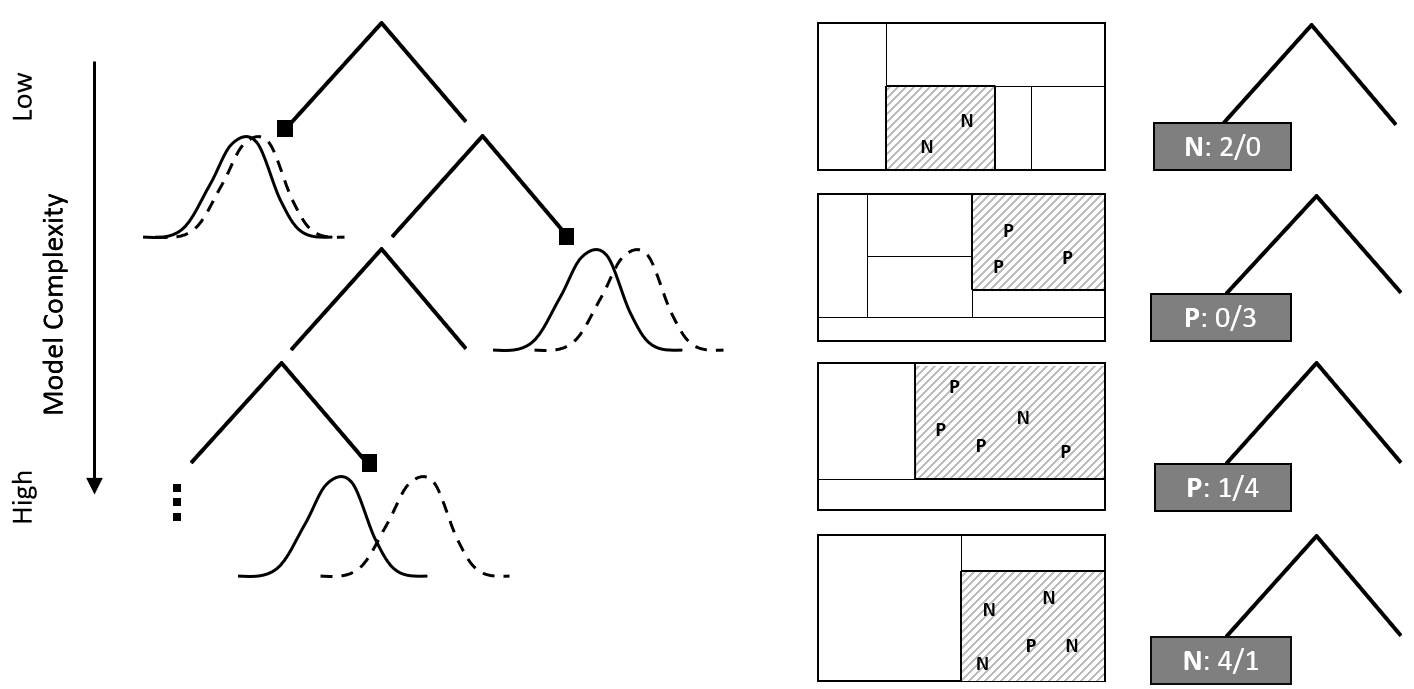
\includegraphics[scale=0.40,angle=0]{fig/tree3}
		\label{project}
		\caption{.}
	\end{center}
\end{figure}

\subsection{The Problem of Overfitting}

Overfitting stands out as one of the biggest challenges for machine learning. It is not exclusive to machine learning but rather a fundamental problem across science and is at the very heart of the dangers of statistical inference. Hypothesis \(h\) in \(H\) overfits training data if there exists an alternative hypothesis \(\bar{h}\) in \(H\) such that \(errorTrain(h) < errorTrain(\bar{h})\) and \(errorD(h) > errorD(\bar{h})\), where \(errorTrain(h):=\) error of hypothesis \(h\) over training data and \(errorD(h):=\) error over entire distribution \(D\) of data. A hypothesis overfits the training examples if some other hypothesis that fits the training examples less well actually performs better over the entire distribution of instances [1].

When overfitting occurs, the learned hypothesis is very good at calculating the answers for the given data, but much less so for new instances it encounters. In a sense, the machine learning algorithm has become fixated on unimportant features of the training data overlooking the big picture. It often occurs when the algorithm has too many options to play with in designing its mappings, an approximation of the target function. The freedom to tune parameters and add complexity until it exactly matches the training data, rather than looking for large, systematic patterns leads to high variance [6].

The expected prediction error at any given data point \(x_0\), the generalization error, can be decomposed as follows [5]: 
\begin{align*}
Err(x_o) &= \EX[(Y - \bar{f}(x_0))^2 \mid X = x_0] \\
& =  \sigma^2_\epsilon + [\EX\bar{f}(x_0) - f(x_0)]^2 + \EX[\bar{f}(x_0) - \EX\bar{f}(x_0)]^2\\
& =  \sigma^2_\epsilon + Bias^2(\bar{f}(x_0)) + Var(\bar{f}(x_0)) \\
& = Irreducible Error + Bias^2 + Variance
\end{align*}

The bias and variance terms make up the error of \(\bar{f}(x_0)\) in estimating \(f(x_0)\). The bias component is the squared difference between the true mean \(f(x_0)\) and the expected value of the estimate \([\EX\bar{f}(x_0) - f(x_0)]^2\), where the expectation averages the randomness in the training data. The variance term refers to the amount by which the estimate of the target function would change if it was estimated using a different training data set. Ideally the estimate for the underlying pattern should not vary too much between training sets. More generally, as the model complexity is increased, the variance tends to increase and the squared bias tends to decrease. The opposite behavior occurs as the model complexity is decreased. The first term in this expression is the irreducible error, a combination of stochastic and deterministic noise. More precisely, stochastic noise are fluctuations or measurement errors that can not be modelled. Re-measuring \(y_n\) changes this component. Deterministic noise is the part of the target function that can not be represented. Changing \(H\) changes this component. With a single dataset \(D\) and fixed \(H\) it is impossible to distinguish [6].  

PU learning is a semi-supervised technique that does not make the simplifying assumption of GBS instances being negative. Instead, a one-class classifier is trained on GESIS only. [...] This can result in even better assessment. [Read Literature] - Imporance weighted cross validation and pu learning with proper assessment.

For further, more technical reading, references to background papers are provided in [38].

Overfitting stands out as one of the biggest challenges for machine learning. It is not exclusive to machine learning but rather a fundamental problem across science and is at the very heart of the dangers of statistical inference. By definition, statistical inference is taking the results of applying some sort of construct or model to specific data and then speculating that it would continue to perform well beyond the original observation range.

State-of-the-art techniques in positive-unlabeled learningtackle this problem by treating the unlabeled sample as neg-atives and training a classifier to distinguish between la-beled (positive) and unlabeled examples. 
Surprisingly,for a variety of performance criteria, non-traditional classi-fiers achieve similar performance under traditional evalua-tion as optimal traditional classifiers (Blanchard et al. 2010;Menon et al. 2015). 
	
\section{Discriminative Learning}

\begin{table}[ht] 	
    \begin{center}
            {\footnotesize
            \begin{tabular}{l|cccccccccc}
                \hline \hline
                           &  TP Rate & FP Rate & Precision & Recall & F-Measure & ROC Area & PRC Area & Class \\
                \hline
                      & 0.000 & 0.000 & ? & 0.000 & ? & 0.500 & 0.130 & GBS &\\
                      & 1.000 & 1.000 & 0.870 & 1.000 & 0.931 & 0.500 & 0.870 & GESIS &\\
                \hline \hline
		 W. Avg. & 0.870 & 0.870 & ? & 0.870 & ? & ? & 0.500 & 0.774 &
            \end{tabular}}
        \caption{Some descriptive statistics of location and dispersion for 2100 observed swap rates for the period from February 15, 1999 to March 2, 2007. Swap rates measured as 3.12 (instead of 0.0312). See Table \ref{Tab:DescripStatsRawDataDetail} in the appendix for more details.}
\label{Tab:DescripStatsRawData}
\end{center}
\end{table}

\section{Learning from Positive and Unlabeled Data}

Breiman [9] introduced bagging as a technique to construct strong ensembles by combining a set of base models. Breiman [10] stated that “the essential problem in combining classifiers is growing a suitably diverse ensemble of base classifiers” which can be done in various ways [12]. In bagging, the ensemble models use majority voting to aggregate decisions of base models which are trained on bootstrap resamples of the training set. From a Bayesian point of view, bagging can be interpreted as a Monte Carlo integration over an approximated posterior distribution [40]. 

In his landmark paper, Breiman [9] noted that base model instability is an important factor in the success of bagging which led to the use of inherently instable methods like decision trees in early bagging approaches [19, 11]. The main mechanism of bagging is often said to be variance reduction [4, 10]. In more recent work, Grandvalet [24] explained that base model instability is not related to the intrinsic variability of a predictor but rather to the presence of influential instances in a data set for a given predictor (so-called leverage points).
The effect of bagging is explained as equalizing the influence of all training instances, which is beneficial when highly influential instances are harmful for the predictor’s accuracy.

We have shown the effect of resampling contaminated sets and provided some basic insight into the mechanics of bagging. We will now link these two elements to justify bagging approaches in the context of contaminated training sets. Its usefulness can be considered by both the variance reduction argument of Bauer and Kohavi [4] and equalizing the influence of training points as described by Grandvalet [24]. Variance reduction. Resampling a contaminated set yields different levels of contamination in the resamples as explained in Section 3.1. Varying the contamination between base model training sets induces variability between base models without increasing bias. This observation enables us to create a diverse set of base models by resampling both P and U. The variance reduction of bagging is an excellent mechanism to exploit the variability of base models based on resampling [4, 10]. In the context of RESVM, a tradeoff takes place between increased variability (by training on smaller resamples, see Figure 1) and base models with increased stability (larger training sets for the SVM models). (https://arxiv.org/pdf/1402.3144.pdf)

\hfill \\

\begin{algorithm}[H]
\noindent\rule{12cm}{1.1pt}
\caption{PU training procedure}\label{alg:alg1}
\KwIn{\(P\): set of positive instances (GESIS)}
\myinput{\(U\): set of unlabeled instances (GBS)}
\myinput{\(n_{models}\): number of base models in ensemble}
\myinput{\(n_P\): size of bootstrap sample of \(P\)}
\myinput{\(n_U\): size of bootstrap sample of \(U\)}
\KwResult{Scoring function \(f:U \rightarrow \) $\mathbb{R}$}
\noindent\rule{6cm}{0.4pt}\\
Initualize: 
\(f(x) \leftarrow 0\) and 
\(c(x) \leftarrow 0\)\\
\For{t = 1 to \(n_{models}\)}{
\hfill \\
  Draw a bootstrap sample \(P_t\) of size \(n_P\). \\
  Draw a bootstrap sample \(U_t\) of size \(n_U\). \\
  Train classifier \(f_t\) to discriminate \(P_t\) against \(U_t\). \\
  For any \(x \in U \backslash U_t\), update:
\[f(x) \leftarrow f(x) + f_t(x),\]
\[c(x) \leftarrow c(x) + 1\]
}
Return \[s(x) = f(x)/c(x)\]
\hfill \\

\end{algorithm}

\begin{comment}
\begin{algorithm}[H]
\caption{Transductive bagging PU learning}\label{alg:alg2}
\KwIn{\(P\): set of positive instances (GESIS)}
\myinput{\(U\): set of unlabeled instances (GBS)}
\myinput{\(K_P\): size of bootstrap samples, \(T\): number of base models in ensemble}
\KwResult{Ranking score \(s:U \rightarrow \) $\mathbb{R}$}

\For{t = 1 to \(T\)}{
 Draw a bootstrap sample \(P_t\) of size \(K_P\). \\
 Train classifier \(f_t\) to discriminate \(P_t\) against \(U\). \\
 For any \(x \in U \backslash U_t\), update:
\[f(x) \leftarrow f(x) + f_t(x),\]
\[n(x) \leftarrow n(x) + 1\]
}
Return \[s(x) = f(x)/n(x)\]

\end{algorithm} 
\end {comment}

\subsection{Recovering Model Performance}

methods to estimate true classificationperformance. 

be recov-ered with the knowledge of class priors

results in biased empirical estimates of the classifier performance
now can be corrected with the knowledge of class priors
using the One-Class SVM and its ability to capture the shape of the data set, hence performing better when the data is strongly non-Gaussian, i.e. with two well-separated clusters;

The ROC curve provides in-sight into trade-offs between the classifier’s accuracies onpositive versus negative examples over a range of decisionthresholds. 
(pr-rc) curve, a plot of precision as a function of recall.The precision-recall evaluation, including summary statis-tics derived from the pr-rc curve, may be preferred to ROCcurves when classes are heavily skewed (Davis and Goad-rich 2006).Although model learning and performance evaluation in asupervised setting are well understood (Hastie et al. 2001),the availability of unlabeled data gives additional optionsand also presents new challenges. A typical semi-supervisedscenario involves the availability of positive, negative and(large quantities of) unlabeled data. Here, the unlabeled datacan be used to improve training (Blum and Mitchell 1998) orunbias the labeled data (Cortes et al. 2008); e.g., to estimateclass proportions that are necessary to calibrate the modeland accurately estimate precision when class balances (butnot class-conditional distributions) in labeled data are notrepresentative (Saerens et al. 2002). This is often the casewhen it is more expensive or difficult to label examples ofone class than the examples of the other. 

The intuition for these results comesfrom the fact that in many practical situations, the posteriordistributions in traditional and non-traditional setting pro-vide the same optimal ranking of data points on a given testsample (Jain et al. 2016; Jain, White, and Radivojac 2016).

Such perfor-mance estimation often involves computing the fraction(s)of correctly and incorrectly classified examples from bothclasses; however, in absence of labeled negatives, the frac-tions computed under the non-traditional evaluation are in-correct, resulting in biased estimates. Figure 1 illustratesthe effect of this bias by showing the traditional and non-traditional ROC curves on a handmade data set. Becausesome of the unlabeled examples in the training set are infact positive, the area under the ROC curve estimated whenthe unlabeled examples were considered negative (non-traditional setting) underestimates the true performance forpositive versus negative classification (traditional setting).This paper formalizes and evaluates performance estima-tion of a non-traditional classifier in the traditional settingwhen the only available training data are (possibly noisy)positive examples and unlabeled data.

Though the efficacy of non-traditional classifiers has beenthoroughly studied (Peng et al. 2003; Elkan and Noto 2008;Ward et al. 2009; Menon et al. 2015), estimating their trueperformance has been much less explored.

the widely-accepted evaluation approaches us-ing ROC or pr-rc curves are insensitive to the variation ofraw prediction scores unless they affect the ranking.

Let \(f\) be the true distribution over the input space \(X\) from which unlabeled data is drawn. With distributions f1 and f0 of the positive and negative examples, respectively, it follows that
\[f(x) = \alpha f_1(x) + (1-\alpha)f_0(x)\]
with positive class prior \(\alpha \in [0,1], x \in X\).

Consider the binary classification problem from input \(x \in X\) (BFI-10 and BRS data) to output \(y \in Y\) (representative: '\(1\)', not representative: '\(0\)'). The learning objective is to discriminate between \(X_p\) drawn according to \(f_1\) and \(X_u\) drawn according to \(f\)  and recover its performance estimate in the traditional setting, i.e. evaluating the decision boundary between positive and negative data.

The two main criteria considered in this work are the area under the ROC curve (AUC) and the F-Measure. The ROC curve plots the true positive rate (recall) of a classifier as a function of its false positive rate (Fawcett 2006) over a range of decision thresholds. 
Furthermore, AUC has a meaningful probabilistic interpretation that is used to  the ability of the classifier to separate classesand is often used to rank classifiers (Hanley and McNeil1982). 
Another important performance criterion generallyused in information retrieval relies on the precision-recall 

 The most extensively studied and widely used performance evaluation in binary classification involves estimating the Receiver Operating Characteristic (ROC) curve t

Recall \(\gamma\), FPR \(\eta\) and Precision \(\rho\) are defined as:

\begin{equation*}
\begin{split}
\gamma = P[\hat{Y} = 1| Y = 1] \\
\eta = P[\hat{Y} = 1| Y = 0] \\
\rho = P[Y = 1| \hat{Y} = 1]
\end{split}
\end{equation*}

where \(\hat{Y}\) is an estimate of the true class label \(Y\).

TPR \(\gamma\) can be estimated directly, because \(X_p\) was sampled from \(f_1\), while this does not hold true for \(\eta\) given the absence of samples from \(f0\).

\begin{gather*}
\gamma = \e{f_1[h(x)]} = \frac{1}{|X_p|} \sum\nolimits_{x \in X_p} h(x) \\
\hat{\eta}^{pu} = \e{f[h(x)]} = \frac{1}{|X|} \sum\nolimits_{x \in X} h(x) \\
\end{gather*}

The area under precision-recall curves \(AUPR\) can be expressed using the approximated value for the fraction of positives \(\alpha\) in \(X_u\)
\[\rho = \frac{\alpha \gamma}{\hat{\eta}^{pu}}\]

The area under ROC curves \(AUROC^{pu}\) so far could only be estimated for the positive versus unlabeled classification by plotting \(\gamma\) and \(\hat{\eta}^{pu}\). To calculate \(AUC\) from \(AUC^{pu}\), S. Jain et al. (2015) express \(\eta\) in terms of \(\hat{\eta}^{pu}\) and \(alpha\) and provide a full derivation from the probabilistic definition of the AUC with

\[\eta = \frac{\hat{\eta}^{pu} - \alpha \gamma}{1 - \alpha}\] so that

\[AUC = \frac{AUC^{pu} - \frac{\alpha}{2}}{1 - \alpha}\] proving

\[AUC > AUC^{pu} \iff AUC^{pu} > \frac{1}{2}\]

\section{Artificial Data Synthesis}

Try to avoid giving the synthesized data properties that makes it possible for a learning algorithm to distinguish synthesized from non-synthesized example such as if all the synthesized data comes from one of 20 car designs, or all the synthesized audio comes from only 1 hour of car noise. This advice can be hard to follow. 

\begin{figure}[ht]
	\begin{center}
		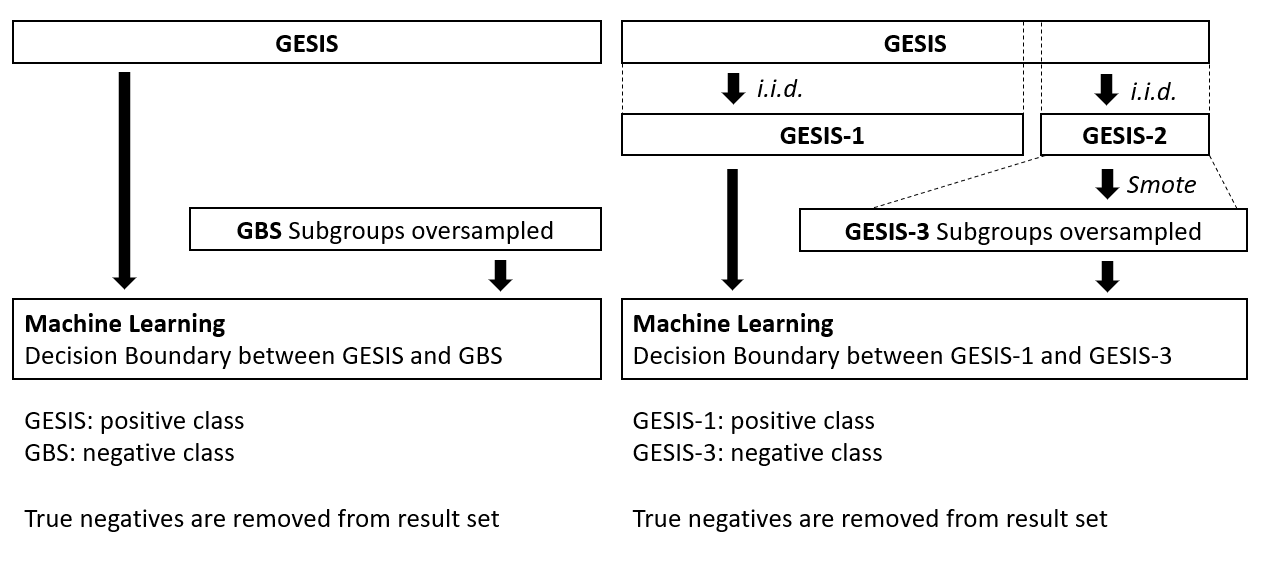
\includegraphics[scale=0.52,angle=0]{fig/procedure}
		\label{std}
	\end{center}
\end{figure}


